\documentclass[titlepage]{article}
\usepackage[utf8]{inputenc}
%%%%%%%%%%%%%%%%%%%%%%%%%%%%%%%%%%%%%%%%%%%%
% ------ Packages ------
\usepackage{fullpage}           %sets margins to 1"
\usepackage{titling}
\usepackage[none]{hyphenat}     %NO HYPHENS
\usepackage[toc,page]{appendix}

\usepackage{tikz}               %graphics
\usepackage{framed}             %boxes in figures
\usepackage{multicol}           %columns
\usepackage{hyperref}           %links
\usepackage{amsmath,amstext}    %math
\usepackage{amsfonts}           %math fonts
\usepackage{mathtools}
% \usepackage{minted}             %code
\usepackage[parfill]{parskip}   %lineskip instead of indent
% \usepackage{gensymb}

\usepackage{caption}
\usepackage{subcaption}

\DeclarePairedDelimiter\ceil{\lceil}{\rceil}
\DeclarePairedDelimiter\floor{\lfloor}{\rfloor}



%%%%%%%%%%%%%%%%%%%%%%%%%%%%%%%%%%%%%%%%%%%%

%%%%%%%%%%%%%%%%%%%%%%%%%%%%%%%%%%%%%%%%%%%%
% ------ Package Preferences ------
\setlength{\droptitle}{-2cm}

\graphicspath{ {Images/} }

\hypersetup{                %color of links
    colorlinks,
    linkcolor=red,
    urlcolor=blue
}

\def\UrlBreaks{\do\/\do-} %url line breaks
%%%%%%%%%%%%%%%%%%%%%%%%%%%%%%%%%%%%%%%%%%%%

%%%%%%%%%%%%%%%%%%%%%%%%%%%%%%%%%%%%%%%%%%%%
% ------   Macros   ------
\renewcommand{\thesubsection}{\thesection.\alph{subsection}} %subsections to letters
\renewcommand{\thesubsubsection}{\thesubsection.\roman{subsubsection}}

\newcommand{\dline}{\hrule \vskip -.2em \hrule} % double line

%%%%%%%%%%%%%%%%%%%%%%%%%%%%%%%%%%%%%%%%%%%%

%%%%%%%%%%%%%%%%%%%%%%%%%%%%%%%%%%%%%%%%%%%%
% ------ Title Block ------
\title{A review of modern bone trauma analysis\\ \large Forensic Anthropology, Wellesley College}
\author{Sophia Li}
\date{\today \\ \vspace{5em}}

%%%%%%%%%%%%%%%%%%%%%%%%%%%%%%%%%%%%%%%%%%%%


\begin{document}

% ------ Pre-Content ------
\maketitle

% ------   Content   ------

\section{Introduction}
This review paper aims to be a comprehensive summary of modern bone trauma analysis. It will begin with a section detailing bone physiology and bio-mechanics, specifically regarding changes to the material properties of the bone as the body decomposes. Additionally, it will summarize methods of determining ante-mortem trauma on the bone to peri/post-mortem trauma by examining the healing exhibited at the trauma site.

Additionally, as the approach to an investigation based on the type of trauma differs depending on the type of trauma observed on the bone, this paper will give a summary of current methods of identification and investigation for the five major types of bone trauma. These include ballistic, blast, blunt force, sharp force, and thermal trauma. Each section will begin with a description on the characteristics of the trauma, and methods of identification. It will follow with an overview of the current methods used in the medico-legal system to identify the tool used and the nature of the trauma event based on evidence found in the bone.

This paper will conclude with a discussion on the future of bone trauma analysis, and why trauma analysis is important to forensic anthropologists in the field today.

\section{Material properties of bone}
The human skeleton is the constantly changing frame of the body, with cell turnover ensuring that the bone will be able to grow, heal, and adapt. There are two main types of bone tissue, specifically cortical bone and cancellous bone (synonmyous with trabecular bone). Cortical bone forms the hard hollow cylinder of the bone and is responsible for mechanical stability. Cancellous bone is the spongy interior of the cylinder, and is responsible for nutrient storage and transport. The tissues are biologically identical, but differences in the arrangement of the microstructure results in different material properties. Cortical bone forms about 80\% of the mass of the skeleton, and forms a hollow cynlinder within which the spongy cancellous bone resides. \cite{bone} Due to the difference in material properties between cortical and cancellous bone, the ratio of of the two at a trauma site will affect the definition of the mark left behind. Fig.\ref{fig:bone_struct} provides a cross-sectional view of the two types of ossesous tissue in an adult femur and provides numerical stress thresholds for adult bone.

\begin{figure}[h!]
\centering
\begin{subfigure}{.5\textwidth}
  \centering
  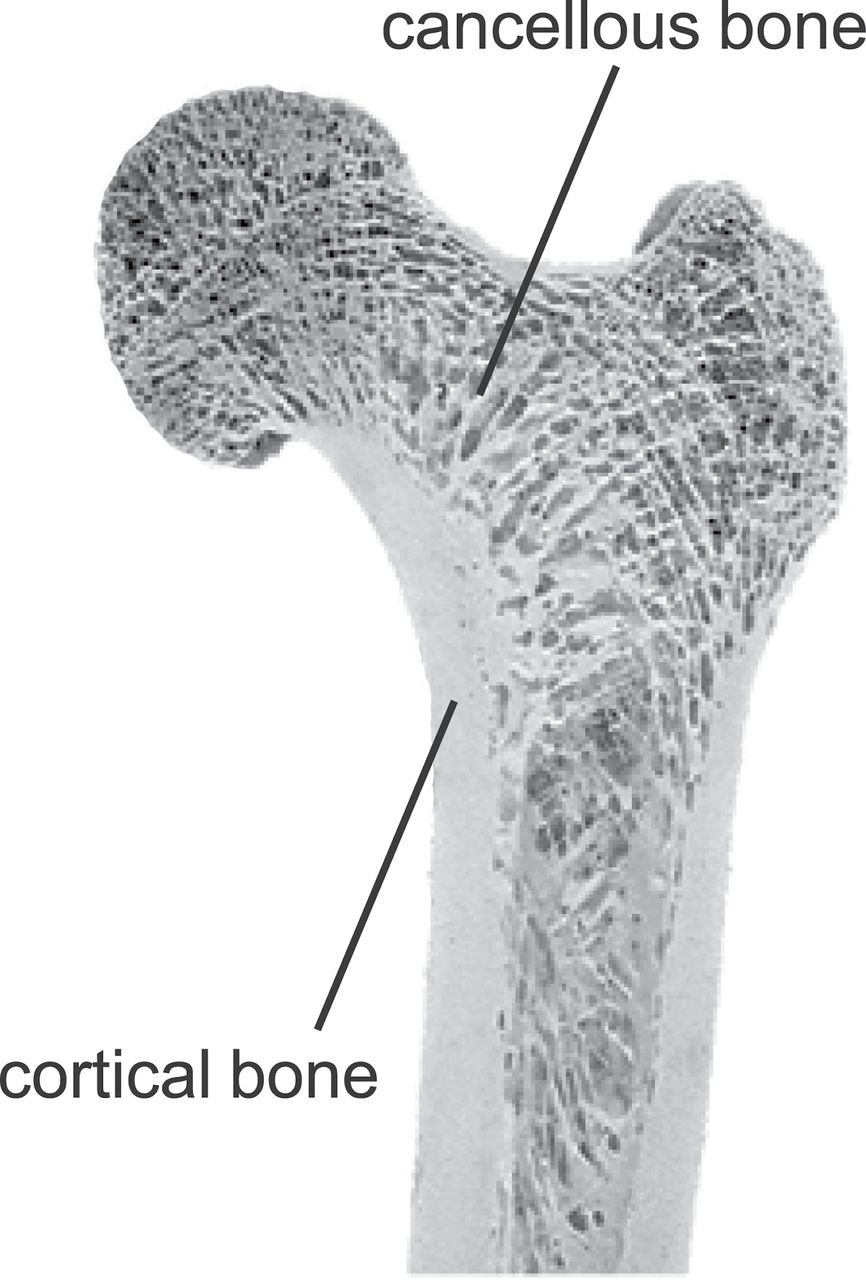
\includegraphics[width=.5\linewidth]{img/bone_microstructure}
  \end{subfigure}%
\begin{subfigure}{.5\textwidth}
  \centering
  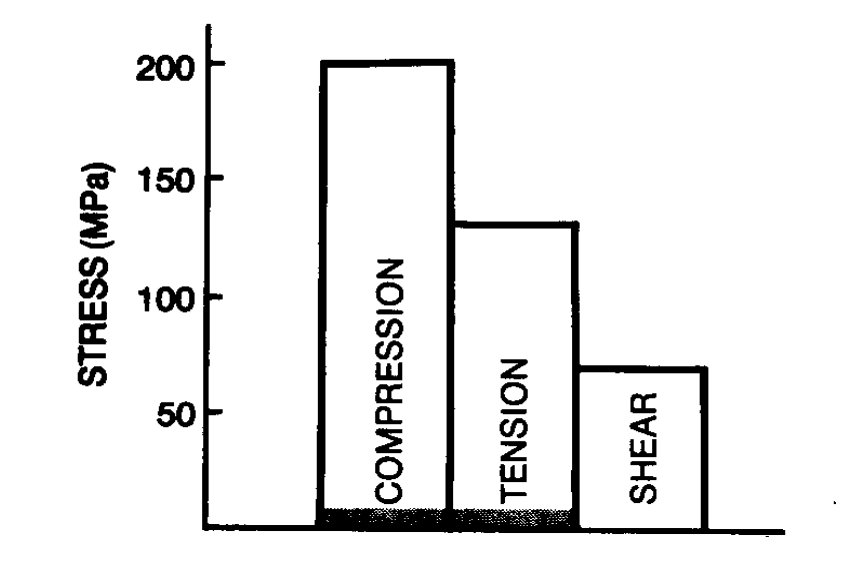
\includegraphics[width=1.1\linewidth]{img/bone_stress}
  \caption{}
\end{subfigure}
\caption{(a) is a cross-section of a human femur, showing the difference between cancellous and cortical bone. (b) charts ultimate stress thresholds for adult cortical bone. Shaded areas indicate thresholds for cancellous bone.}
\label{fig:bone_struct}
\end{figure}

Bone is considered anisotrophic, as bone trauma will be exhibited differently based on the location of the impact. However, we can observe the following:

Crack propagation happens more readily in the lateral direction due to the organization of the bone tissue fibers. \cite{mechanics}

%TODO: INSERT IMAGES OF CRACKS

Bone is strong against compression and tension stress, but weak against shear force. This is consistent with typical loading forces bone experiances in day to day life. However, most cases of bone trauma seen in a forensic context is due to shear force.

%TODO: INSERT CHART OF STRESS

The bio-mechanics of a specific sample of bone depend heavily on the sampled individual. Factors like age, sex, location in body, and amount of water present will heavily affect the mechanical properties of the bone. Water content is especially important in a forensic context, as it will allow investigators to determine whether bone trauma occured ante, peri, or post-mortem as water evaporates as the body decomposes.

Forensic investigators interested in timing trauma observed on the bone should observe the following characteristics.

\subsection{Ante-mortem trauma}
Ante-mortem trauma refers to trauma on the skeleton that occurs prior to the death of the individual. In-vivo bone exhibits recovery, in the form of (INSERT TERMINOLOGY HERE).

\subsection{Peri-mortem trauma}
Peri-mortem trauma refers to trauma that occurs around the death of the individual.

\subsection{Post-mortem trauma}
Trauma after death of the individual.

\newpage
\section{Ballistic}
Ballistic trauma on bone is usually the result of a bullet, though it may be applied to any fast traveling object that has collided with bone. Features that indicate possible ballistic trauma include the presence of the projectile that can be associated with bone, and fracture patterns corresponding to a high velocity impact. Because ballistic trauma in cases where a forensic anthropologist may be bought in are almost always due to a bullet, this section will only examin ballistic trauma in the case of a bullet.

The bullet enters the wound with a higher velocity than when it exits, thus the entrace wound will usually be smaller than the exit wound. Entrace wounds can be identified by looking at beveled edges towards the interior of the body. As the bullet exits the wound, it hits the bone with less force causing shattering and greater fractures to the internal tissue.

\newpage
\section{Blast}

\newpage
\section{Blunt force trauma}
While ballistic and blast trauma can both be techinically classified as blunt force trauma, in the context of this paper we will refer to blunt force trauma as trauma resulting from a low-velocity impact from a blunt object, or a low-velocity impact with a blunt surface.

Due to the low-velocity impact, features suggesting blunt force trauma include plastic deformation, lamination, tool marks/impressions at trauma site, or fracture patterns on the bone suggesting low velocity impact.\cite{trauma}



\newpage
\section{Sharp force trauma}
Sharp force trauma is characterized by trauma resulting from a tool that is edged, pointed, or beveled. Features indicating sharp force trauma on bone include straight-lined incisions, punctures or gouges, clefs or kerfs. Considerations must be taken when examining the wound, since alterations to the bone like scrapes or score marks are not classified as sharp force trauma. \cite{trauma}

(SECTION DESCRIBING EACH TYPE OF TRAUMA i.e gouges, clefs, kerfs)

There are a few methods currently used in examining bones with evidence of sharp force trauma. Casting is an immediately viable option, and is a non-destructive way of providing investigators a method of examining the wound. However, casting on on soft-tissue has been met with mixed success, and is unable to provide information to investigators on the micro scale about the incision. However, it is possible to estimate the motion of the tool based on whether it is a slash (the incision is wider than it is deep), or a stab (the incision is deeper than it is wide) through visual inspection. \cite{serrated} Macro inspection of the wound at a visual scale can qualitatively describe the tool used in the trauma down to a class, such as \"single edged\" or \"beveled\". The handedness of an attacker, or whether a wound is self inflicted can be determined by the angle of the incision in context to the position of the body.

Micro-CT scanning technology is used to give greater insight to the patterned marks left within bone from sharp force trauma, by giving investigators cross-sectional view of the impact site. Tests conducted via sharp force inpact analyzed by micro-CT scanning were able to correctly determine the size and shape of a knife, in addition to the angle of impact in most cases. The tests were not quite as accurate when the knife was excessively rocked or rotated within the bone, though examining the wound profile and the tip of the knife allows better precision.\cite{micro-ct}

\newpage
\section{Thermal}
Thermal damage to bones

\newpage
\bibliographystyle{ieeetr}   % this means that the order of references
			    % is dtermined by the order in which the
			    % \cite and \nocite commands appear
\bibliography{mybib.bib}

\end{document}
\end{document}
